人地关系是人类活动与地球表层系统的关系\cite{wu1991,li2016d}。
地球表层系统是一个复杂的开放系统,四个圈层之间存在复杂的能量交换和物质流动,人类不能脱离其他任何圈层,人类的活动也会影响其他圈层,从而深远地影响水圈。
参照上述定义时,“人-地”与“人-水”都将指向人类和地球表层系统共同构成的复合系统,因此人水关系不能被简单地定义为“人类活动与水圈的关系”。
在实际研究中,研究者绝无可能穷尽此人水系统的全部作用关系,通常会针对系统的某个影响/反馈“实体”,给出$Y = f(X_1, X_2, \dots)$的显式表达,因此出于研究需要,本章为广义的“人水关系”给出如下定义(图\ref{ch2:fig:definitions}):

{\kai~人类活动直接改变水圈要素、过程,或水圈要素、过程是影响不可被忽略的变量时,人与地球表层系统的相互作用。}

本研究关注人水关系的演变过程,因为人水关系并非仅在人类有能力影响水圈后才出现。
人类活动改造水圈或水文系统是人水关系的一种表现形式,相关研究(如流域的“自然-社会”二元水循环理论)主要关注的是近代人类活动对水圈要素过程的影响\cite{wang2006, wang2016}。
水还是塑造人类世界观和行为模式的重要元素,相关研究(如社会科学中的“水的社会性”研究)也属于广义的人水关系。
因本研究旨在服务流域可持续性,因此不再考虑人类对水圈影响微乎其微的史前时期,仅将时间尺度限制在人类有能力改造水圈要素过程的时期。

% 开题报告
\begin{figure}[!htb]
    \centering
    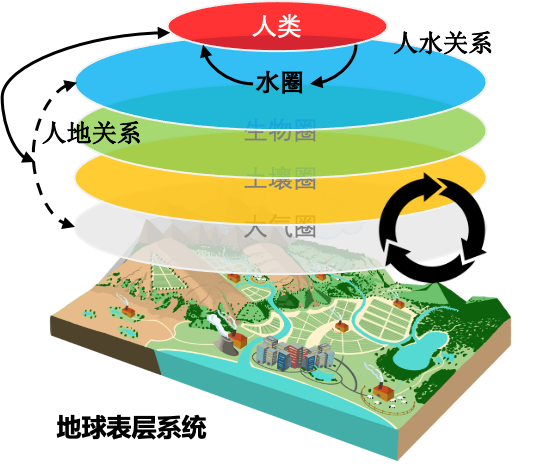
\includegraphics[width=0.6\textwidth]{img/ch2/ch2_scope.png}
    \caption[广义人水关系的概念内涵示意图]{广义人水关系的概念内涵示意图。人类活动直接改变水圈要素、过程,或水圈要素、过程是影响不可被忽略的变量时,人与地球表层系统的相互作用。}\label{ch2:fig:definitions}
\end{figure}

% 主要研究内容与相关概念。本研究主要关注的人-水系统(Human-water system)与概念范围更广的社会-生态系统(Social-ecological system, SES)都是典型的复杂系统(Complex system),因此基于复杂系统的建模也常常以人-水系统为研究对象。(a)本研究首先以黄河为研究案例,梳理人-水系统演变过程;(b)在其基础上重点分析水的资源属性下发生变化的人-水关系。(c)最后在SES分析框架下,利用基于复杂系统建模的技术手段,对资源属性引导下的人-水关系演变过程进行机制模拟。

关系是指将两个或多个概念或对象相连的方式或状态。在本研究中,“人水关系”是指在给定的时空尺度下,利益相关者(个体、组织、或集体)基于自身利益,通过决策与地球表层系统中水圈的要素和过程相连接的状态~\cite{bonnafous-boucher2016}。
利益相关者是指在一个系统或事件中存在利益关系的个人、团体、组织,可以来自系统内部或外部,并受到系统变化的直接或间接影响~\cite{bonnafous-boucher2016}。
简而言之,本研究关注的“人水关系”不是人类活动生产的水库、大坝、污染物、法律制度等,而是利益相关者通过相关的决策过程,而与地球表层水圈变量相互连接的状态。
利益相关者的决策过程通常与其成本-收益有关,他们通过考虑潜在损失和收益来决定是否修堤防洪、建造水库、进行取水等活动,这种“人”与“水”之间的连接模式就是本研究定义的“人水关系”:

{\kai~在给定的时空尺度下,利益相关者(个体、组织、或集体)基于自身利益,通过决策与地球表层系统中水圈的要素、过程相连接的状态。}
